%%%%%%%%%%%%%%%%%%%%%%%%%%%%%%%%%%%%%%%%%%%%%%%%%%%%%%%%%%%%%%%%%%%%%
%  Executar:   pdflatex
%              bibtex
%              pdflatex
%              pdflatex
%%%%%%%%%%%%%%%%%%%%%%%%%%%%%%%%%%%%%%%%%%%%%%%%%%%%%%%%%%%%%%%%%%%%%
%  WSTeX: Template LaTeX para formatação de trabalhos científicos 
%  TCC, Mestrado e Doutorado segundo as normas ABNT
%%%%%%%%%%%%%%%%%%%%%%%%%%%%%%%%%%%%%%%%%%%%%%%%%%%%%%%%%%%%%%%%%%%%%
% Aviso de Direitos Autorais:
%
% Este template LaTeX é protegido por direitos autorais e foi 
% disponibilizado para seu uso pessoal e/ou educacional pelo autor. 
% Qualquer alteração, reprodução ou distribuição deste template, no 
% todo ou em parte, sem consentimento expresso do autor é 
% estritamente proibida e sujeita às leis de direitos autorais 
% aplicáveis.
%
% O autor deste template investiu tempo e esforço significativos na 
% sua criação, visando fornecer uma ferramenta útil e de qualidade 
% para a comunidade acadêmica. Portanto, para garantir o respeito ao 
% seu trabalho e direitos autorais, solicita-se que qualquer 
% modificação, adaptação ou compartilhamento deste template seja 
% feito somente após obtenção do consentimento por escrito do autor.
%
% O não cumprimento destas condições pode resultar em consequências 
% legais, incluindo, mas não se limitando a ações judiciais por 
% violação de direitos autorais.
%
% Agradeço pela compreensão e cooperação no respeito aos direitos 
% autorais e à propriedade intelectual.
%
% Autor: Wladimir Seixas
% email: seixas@ufscar.br
% Versão: 15/05/2025
%%%%%%%%%%%%%%%%%%%%%%%%%%%%%%%%%%%%%%%%%%%%%%%%%%%%%%%%%%%%%%%%%%%%%
%
%  Documento LaTeX baseado na classe REPORT
%  Pacotes LaTeX que já estão carregados:
%
% ifthen      fontenc      mathptmx     textcase    
% inputenc    babel        microtype    geometry   
% setspace    graphicx     float        indentfirst  
% fancyhdr    etoolbox     caption      footmisc   
% enumitem    pdfpages     tocloft      amsmath    
% amsfonts    amssymb      varioref     amsthm      
% imakeidx    hyperref     color        biblatex    
% appendix    mdframed     acronym
%
%    Arquivos: wstex.cls (template LaTeX)
%              monografia.tex 
%              referencias.bib (database BibTeX)
%              logos (diretório contendo logos)
%
%%%%%%%%%%%%%%%%%%%%%%%%%%%%%%%%%%%%%%%%%%%%%%%%%%%%%%%%%%%%%%%%%%%%%
%  PREENCHER OS APENAS OS CAMPOS DE INFORMAÇÕES
%  NÃO ALTERAR A ORDEM DOS COMANDOS. 
%  A CONFECÇÃO DO TRABALHO SEGUE A ORDEM DEFINIDA NA ABNT
%  ATENÇÃO: não comentar os ambientes obrigatórios   
%%%%%%%%%%%%%%%%%%%%%%%%%%%%%%%%%%%%%%%%%%%%%%%%%%%%%%%%%%%%%%%%%%%%%

% CURSO          OPÇÃO
% TTC            tcc
% MESTRADO       mestre
% DOUTORADO      doutor

% Escolher uma das opções (caso não se aplique mantenha %).
% Opcional: twoside -> impressão do documento frente-verso.
%                      Não utilizar para a versão digital

%\documentclass[tcc]{wstex}
%\documentclass[tcc,licenciatura]{wstex}
%\documentclass[tcc,bacharelado]{wstex}
\documentclass[mestre]{wstex}
%\documentclass[doutor]{wstex}

% Para relatórios de disciplinas e pesquisa
%\documentclass[relatorio]{wstex}

% Personaliza o texto da capa 
%\objetivo{Coloque aqui o seu texto para descrever o relatório.}

% Os hyperlinks serão de cor azul escuro (default).
% Descomente a linha a seguir caso queira os hyperlinks na cor do texto.
% \definecolor{corlink}{rgb}{0,0,0}

% Coloque aqui outros pacotes LaTeX que você faça uso 
% (ver tabela acima)
% \usepackage[•]{•}

\begin{document}

%%%%%%%%%%%%%%%%%%%%%%%%%%%%%%%%%%%%%%%%%%%%%%%%%%%%%%%%%%%%%%%%%%%%%
% DADOS: Preencher os campos comentando caso não se aplique.
%%%%%%%%%%%%%%%%%%%%%%%%%%%%%%%%%%%%%%%%%%%%%%%%%%%%%%%%%%%%%%%%%%%%%

% Instituição 
\instituicao{Nome da Instituição}

% Define o arquivo de logotipo da instituição
\logotipo{./logos/LogoUFSCar}

% Instituto/Centro
\centro{Nome do Centro/Instituto/Faculdade}

% Depto responsável para opção tcc-gradução
%\progresp{Departamento ou Curso} 
% Programa responsável para opção pós-graduação
\progresp{Programa de Pós-Graduação Responsável}

% Área OPCIONAL somente para Mestrado/Doutorado
\area{Área de concentração}

% Ano da defesa depósito
\ano{2025}

% Título do trabalho
\titulo{Título do trabalho}

% Autoria (escolha uma das opções)
% Opção de Gênero -> Mestre/Doutor
%\autor{Nome do autor}
% Opção de Gênero -> Mestra/Doutora
\autora{Nome da autora}

% Orientação - preencha o campo correspondente
% OBS: comente caso utilize a opção "relatorio"
% Escolha uma das opções de gênero
\orientador{Nome do orientador}
%\orientadora{Nome da orientadora}
%\coorientador{Nome da coorientador}
%\coorientadora{Nome da coorientadora}

% Local
\local{Cidade -- UF}

% A capa é um elemento OBRIGATÓRIO 
\capa

%%%%%%%%%%%%%%%%%%%%%%%%%%%%%%%%%%%%%%%%%%%%%%%%%%%%%%%%%%%%%%%%%%%%%
% Elementos pré-textuais
% Parte que antecede o texto com informações que auxiliam na 
% identificação e utilização do trabalho.
%%%%%%%%%%%%%%%%%%%%%%%%%%%%%%%%%%%%%%%%%%%%%%%%%%%%%%%%%%%%%%%%%%%%%

% Folha de Rosto
% A folha de rosto é um elemento OBRIGATÓRIO que apresenta os 
% elementos essenciais para identificação do trabalho.
\cleardoublepage
\folhaderosto

% A ficha catalográfica, elemento OBRIGATÓRIO em trabalhos 
% acadêmicos, segundo a Norma ABNT - NBR 14724/2011 
% (Informação e documentação – Trabalhos acadêmicos – 
% apresentação), deve ser inserida após a folha de rosto no 
% arquivo eletrônico e no verso da folha de rosto na versão 
% impressa. Em ambos os casos na parte inferior da página.
% Se você optar por um lado da folha, a "contagem" deve ser 
% como "folhas". Ex.: 100 f.
% Se você optar por dois lados da folha, “contagem" deve ser
% como "página". Ex.: 100 p.

% Exemplo: https://www.sibi.ufscar.br/servicos/gerador-de-ficha-catalografica
% Para obter a ficha é necessário que o autor preencha os 
% campos com os dados da sua monografia, o programa fará a 
% formatação correta dos dados e irá gerar a ficha 
% catalográfica em um arquivo .PDF, fazendo o download 
% automático.
% Salvar no diretório com o nome "ficha-catalografica.pdf"
% substituindo o arquivo existente,
\fichacatalografica[1]{ficha-catalografica.pdf}

% A folha de aprovação é elaborada e fornecida pela 
% Coordenação de Curso (TCC) ou pelo Programa de 
% Pós-Graduação
% Salvar no diretório com o nome "folha-aprovacao.pdf"
% substituindo o arquivo existente,
% A opção 1.1 aumenta em 10% o tamanho da folha
\folhaaprovacao[1.1]{folha-aprovacao.pdf}

% Dedicatória
% Comente o ambiente a seguir caso não fizer uso.
\begin{dedicatoria}

	A dedicatória é um elemento OPCIONAL em que \\ o autor presta homenagem ou dedica seu trabalho.

\end{dedicatoria}

% Agradecimento
% Comente o ambiente a seguir caso não fizer uso.
\begin{agradecimentos}

	É um elemento OPCIONAL em que o autor faz agradecimentos aos que contribuíram de
	maneira relevante à elaboração do trabalho.

\end{agradecimentos}

% Epígrafe
% É um elemento OPCIONAL em que o autor pode apresentar uma citação. 
% Deve-se fazer a indicação de autoria (citação) e a referência deve 
% constar na lista de Referências no final do trabalho.
% Comente o ambiente a seguir caso não fizer uso.
\begin{epigrafe}

	Epígrafe é um elemento OPCIONAL \\
	Demonstração: Evidente \\
	\textbf{Elon Lages Lima} \cite[p. 154]{elon}.

\end{epigrafe}

% Até 5 palavras-chaves - preencha os campos apropriados
% {1o campo-> em português}{2o campo-> em inglês}
\palavrachaveI{Chave 1}{Key 1}
\palavrachaveII{Chave 2}{Key 2}
\palavrachaveIII{Chave 3}{Key 3}
%\palavrachaveIV{Chave 4}{Key 4}
%\palavrachaveV{Chave 5}{Key 5}

% Resumo na língua vernácula (Português)
\begin{resumo}

	\noindent Elemento OBRIGATÓRIO, deve apresentar os pontos relevantes do texto,
	de forma concisa e que permita uma visão rápida e clara do conteúdo e das
	conclusões do trabalho. Indica-se que o resumo tenha no máximo 500 palavras e
	deve ser elaborado de acordo com ABNT NBR 6028/2003. Deve ser escrito em um
	único parágrafo, sem subdivisões e sem recuo de parágrafo. Abaixo do resumo
	devem ser colocadas as palavras-chave. A indicação Palavra-chave deve ser
	em negrito seguida de dois pontos e espaço. Cada palavra deve ser separada
	uma da outra por ponto final.

\end{resumo}

% Resumo em língua estrangeira (Inglês)
% Versão do resumo em outro idioma para divulgação internacional. É permitido
% colocar o resumo em 1 (um) ou mais idiomas estrangeiros, caso julgue importante
% para divulgação do trabalho. Elaborar o Resumo em língua estrangeira de acordo
% com ABNT NBR 6028/2003. Abaixo do resumo devem ser colocadas as palavras-chave. 
% A indicação Keywords deve ser em negrito seguida de dois pontos e espaço. 
% Cada palavra deve ser separada uma da outra por ponto final.
% Para outra(s) língua(s) que não inglesa --> a ser implementado sob demanda 
% em razão do pouco uso. Entrar em contato com seixas@ufscar.br

\begin{abstract}

	\noindent Version of the abstract in another language for international dissemination. Prepare the abstract in a foreign language accordingly with ABNT NBR 6028/2003. Below the abstract the keywords must be placed. The indication Keywords must be in bold followed by a colon and space. Each word must be separated from each other by a period.

\end{abstract}

% Lista de ilustrações
% Elemento OPCIONAL, precede o Sumário. São consideradas ilustrações: desenhos,
% esquemas, fluxogramas, fotografias, gráficos, mapas, organogramas, plantas,
% quadros, retratos e outras. Recomenda-se criar lista própria, sempre que o número
% de itens ultrapassar 5. Sua construção gráfica é a mesma do Sumário.
% Comente as próximas duas linhas caso não haja ilustrações.
\cleardoublepage
\begingroup
\renewcommand*{\addvspace}[1]{} % Elimina o espaço entre capítulos
\listoffigures
\endgroup

% Lista de Tabelas
% Elemento OPCIONAL elaborada de acordo com a ordem apresentada no texto, tendo
% cada item designado por seu nome específico, acompanhado do respectivo número
% da folha ou página.
% Comente as próximas duas linhas caso não haja tabelas.
\cleardoublepage
\begingroup
\renewcommand*{\addvspace}[1]{} % Elimina o espaço entre capítulos
\listoftables
\endgroup

% Lista de Quadros
% Elemento OPCIONAL elaborada de acordo com a ordem apresentada no texto, tendo
% cada item designado por seu nome específico, acompanhado do respectivo número
% da folha ou página.
% Comente as próximas duas linhas caso não haja quadros.
\cleardoublepage
\begingroup
\renewcommand*{\addvspace}[1]{} % Elimina o espaço entre capítulos
\listofquadros
\endgroup

% Lista de Siglas
% Elemento OPCIONAL com a relação de abreviaturas e siglas utilizadas no texto, 
% seguidas das palavras ou expressões correspondentes, grafadas por extenso. 
% Recomenda-se a elaboração da lista em ordem alfabética.
% Por exemplo, se você usar \ac{UFSCar} pela primeira vez no seu documento, 
% irá aparecer "Universidade Federal de São Carlos (UFSCar)". A partir desse 
% momento, toda vez que usar \ac{UFSCar} em outro lugar do documento, apenas 
% "UFSCar" será impresso. \acs{UFSCar} imprimi apenas a sigla, \acl{UFSCar} 
% imprimir a versão completa e \acf{UFSCar} irá imprimir a versão completa 
% seguida da sigla entre parênteses, independentemente de ser a primeira vez 
% que a sigla é utilizada no texto.
% Comente as próximas sete linhas caso não haja quadros.
\chapter*{Lista de Siglas}
\pagestyle{empty}
\begin{acronym}[XXXXXX]\itemsep 0pt % Espaçamento entre siglas igual ao do documento
	% Defina suas siglas a seguir 
	\acro{BNCC}{Base Nacional Comum Curricular}
\end{acronym}

% Sumário
% Elemento OBRIGATÓRIO que apresenta a enumeração das divisões, seções e outras
% partes do trabalho, na mesma ordem e grafia em que aparecem no texto.
% O Sumário deve ser elaborado de acordo com ABNT NBR 6027/2012.
\cleardoublepage
\pagestyle{empty} % ABNT: Não enumerar as páginas do Sumário
\tableofcontents

% Já estão pré-definidos os seguintes ambientes:
%
%	 \begin{teorema} .... \end{teorema}
%	 \begin{lema} .... \end{lema}
%	 \begin{proposicao} .... \end{proposicao}
%	 \begin{corolario} .... \end{corolario}
%	 \begin{definicao} .... \end{definicao}
%    \begin{axioma} .... \end{axioma}
%	 \begin{conjectura} .... \end{conjectura}
%	 \begin{exemplo} .... \end{exemplo}

% No texto: as ilustrações são elementos gráficos, que servem para complementar
% visualmente o texto e devem ser inseridas próximo ao trecho do texto a que 
% se referem. O número e o título da figura devem vir acima dela, enquanto a 
% fonte deve aparecer embaixo. Se a figura for de elaboração do autor do texto
% colocar
%               Fonte: Elaborada pelo autor.
% Se o autor for do sexo feminino colocar "Elaborado pela autora".
% São enumeradas sequencialmente.
%
% \begin{figure}[H]
%  \begin{center}
%  \caption{<título>}
%  \label{•}
%  \includegraphics[scale=•]{•}
%  \caption*{Fonte: }
%  \end{center}
%  \end{figure}

% No texto: as tabelas são formadas por linhas verticais, devem manter suas bordas
% laterais abertas e geralmente são utilizadas para dados quantitativos. Devem ter: 
% a) um título; b) um cabeçalho; c) um corpo contendo dados numéricos; d) uma linha 
% de fechamento; e) uma fonte; f) notas explicativas, se precisar. O número e o 
% título da tabela devem vir acima dela, enquanto a fonte deve aparecer embaixo.
% São enumeradas sequencialmente.
%
% \begin{table}[H]
%  \begin{center}
%  \caption{<título>}
%  \label{•}
%  \begin{tabular}{•}
%  \end{tabular}
%  \caption*{Fonte: }
%  \end{center}
%  \end{table}
% 
% Os quadros são caracterizados por serem compostos predominantemente por palavras 
% organizadas em linhas e colunas, podendo conter ou não dados numéricos indicativos. 
% Eles se diferenciam das tabelas por apresentarem um conteúdo mais esquemático e 
% descritivo, em vez de estatístico. A apresentação dos quadros é semelhante à das 
% tabelas, exceto pela colocação de traços verticais em suas laterais e pela 
% separação das células. O número e o título do quadro devem vir acima dele, 
% enquanto a fonte deve aparecer embaixo.
% São enumeradas sequencialmente.
% 
% \begin{quadro}[H]
%  \begin{center}
%  \caption{<título>}
%  \label{•}
%  \begin{tabular}{|•|}
%  \hline 
%   ... & ... \\ \hline 
%  \end{tabular}
%  \caption*{Fonte: }
%  \end{center}
%  \end{quadro}

%%%%%%%%%%%%%%%%%%%%%%%%%%%%%%%%%%%%%%%%%%%%%%%%%%%%%%%%%%%%%%%%%%%%%
% Elementos textuais
% O texto é composto pela
%     Introdução, que apresenta os objetivos do trabalho, o
%     Desenvolvimento, que detalha a pesquisa ou estudo realizado e a​ 
%     Conclusão.
%%%%%%%%%%%%%%%%%%%%%%%%%%%%%%%%%%%%%%%%%%%%%%%%%%%%%%%%%%%%%%%%%%%%%

\chapter{Introdução}            %  <<<<---- Pode fazer via \input{file.tex}

Por exemplo, utilizando o acrônimo \ac{BNCC} pela primeira vez no seu documento. A partir desse momento, sempre teremos \ac{BNCC} no documento.

\chapter{Desenvolvimento}       %  <<<<---- Pode fazer via \input{file.tex}

\chapter{Considerações finais}  %  <<<<---- Pode fazer via \input{file.tex}

% \cite[]{} dá a referência.
``Demonstração: Evidente'' \cite[p. 154]{elon}.

Para a citação como sujeito da frase: \textcites{cordeiro} faz diversas considerações sobre a boa redação matemática.

%%%%%%%%%%%%%%%%%%%%%%%%%%%%%%%%%%%%%%%%%%%%%%%%%%%%%%%%%%%%%%%%%%%%%
% Elementos pós-textuais
% Inseridos após a parte textual, apresentam elementos que 
% complementam o trabalho.
%%%%%%%%%%%%%%%%%%%%%%%%%%%%%%%%%%%%%%%%%%%%%%%%%%%%%%%%%%%%%%%%%%%%%

% Referências
% Elemento OBRIGATÓRIO e deve ser elaborada de acordo com ABNT NBR 6023/2002.

% ATENÇÃO: NÃO UTILIZAR O COMANDO \nocite{*}
% TODAS AS REFERÊNCIAS DEVEM SER CITADAS NO TEXTO
% \cite[]{} ou \textcites[]{}

% Utilize o BibLaTeX.
% Colocar as referências no arquivo referencias.bib

% ABNT: As referências devem ser elaboradas em espaço simples, alinhadas à
% margem esquerda do texto e separadas entre si por uma linha em branco
% de espaço simples.
\begin{spacing}{1.0}  % ABNT: espaçamento simples
	\printbibliography
	\addcontentsline{toc}{chapter}{REFER\^{E}NCIAS} % Sumário
\end{spacing}


% Apêndice
% Elemento OPCIONAL que apresenta texto ou documento elaborado pelo autor, a fim de
% complementar sua argumentação. Deve ser precedido da palavra APÊNDICE,
% identificado por letras maiúsculas consecutivas, travessão e respectivo título.
% Comente o ambiente a seguir caso não fizer uso.

\begin{appendices}

	\chapter{Título do Apêndice}

	\section{Seções do Apêndice}

\end{appendices}

% Anexo 
% Elemento OPCIONAL, apresenta um texto ou documento não elaborado pelo autor, que 
% serve de fundamentação, comprovação e ilustração. Deve ser precedido da palavra
% ANEXO, identificado por letras maiúsculas consecutivas, travessão e respectivo
% título.
% Descomente o ambiente a seguir caso fizer uso.

\begin{appendices}
	\renewcommand{\appendixname}{Anexo}
	\setcounter{chapter}{0}

	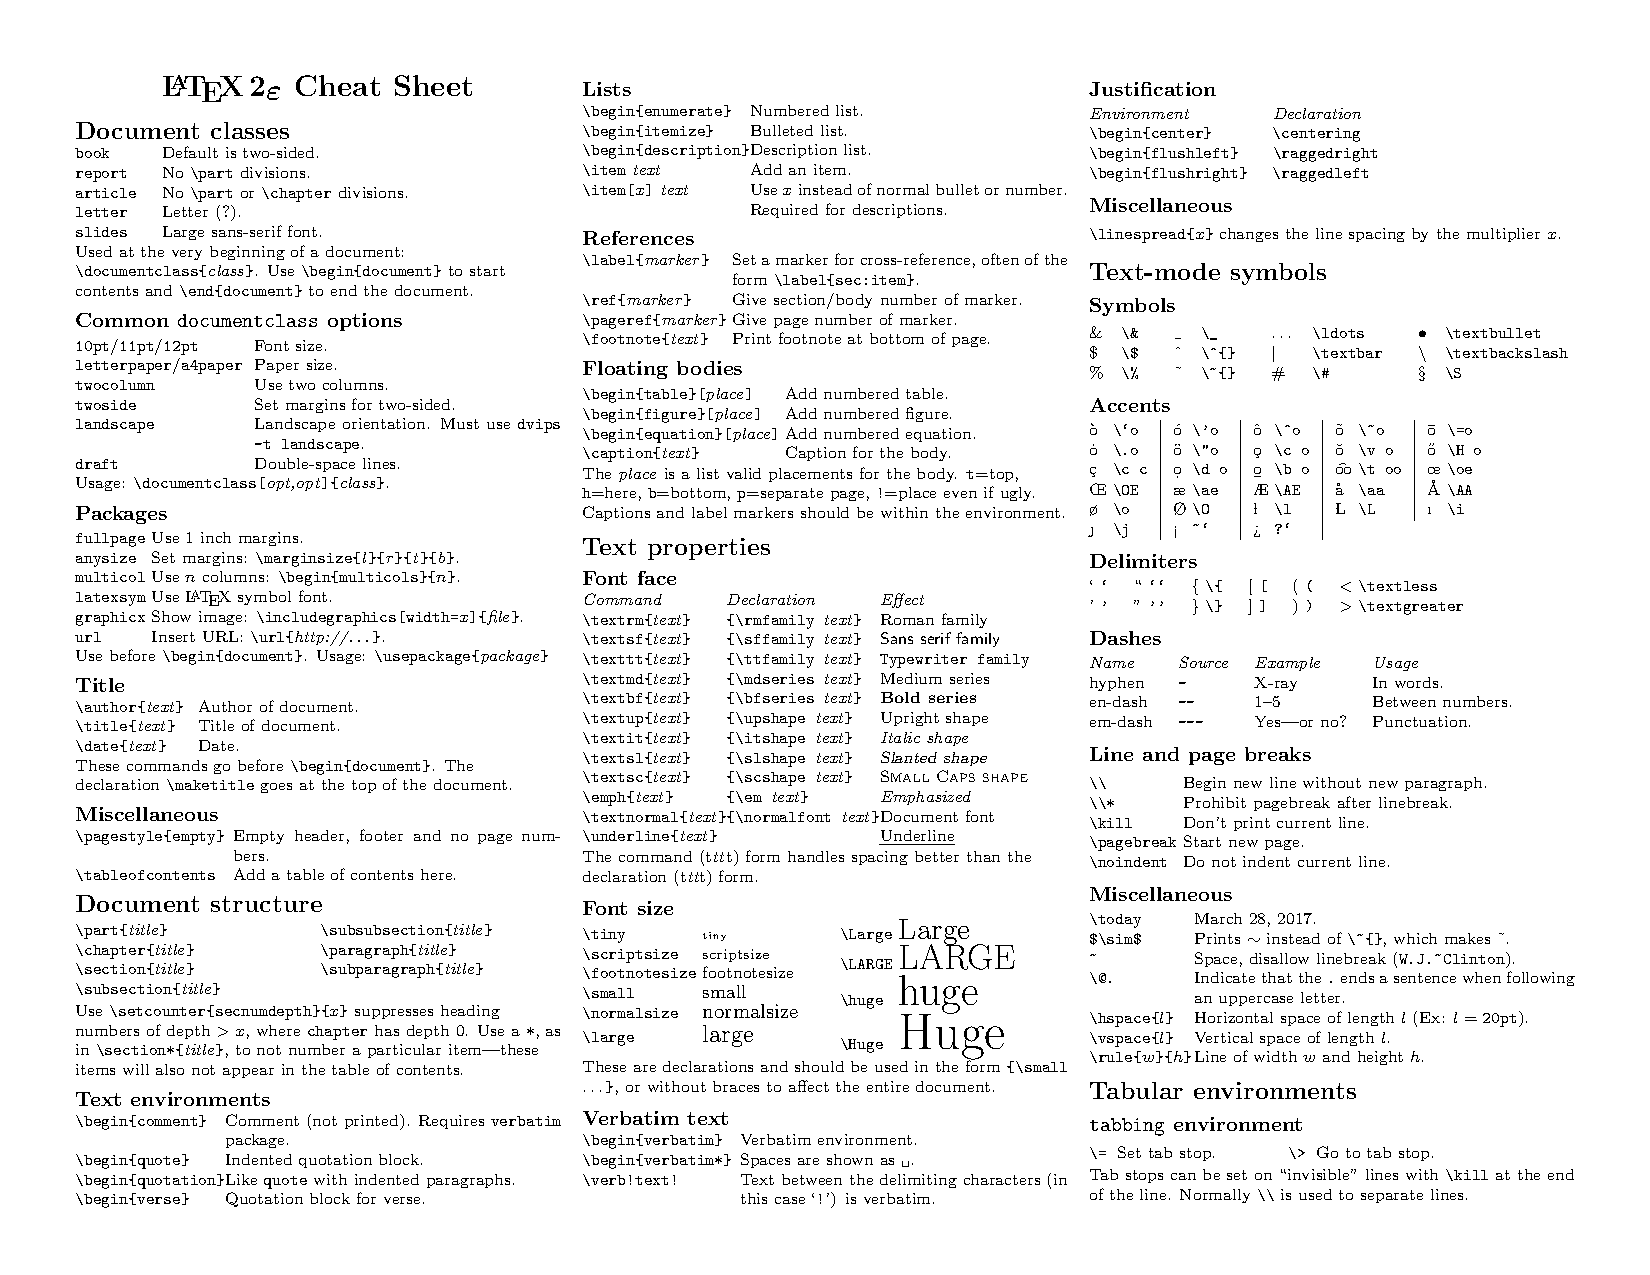
\includepdf[pages=1,width=0.9\textheight,landscape=true,pagecommand={\chapter{Título do anexo} \thispagestyle{fancy} \label{anexo1}} ]{latexsheet.pdf}
	% Caso o arquivo possua mais de uma página
	\includepdf[pages=2,width=0.9\textheight,landscape=true,pagecommand={\thispagestyle{fancy}}]{latexsheet.pdf}

\end{appendices}

% Índice
% Elemento OPCIONAL que apresenta lista de palavras ou frases, ordenadas segundo
% determinado critério, que localiza e remete para as informações contidas no texto.
% Deve ser elaborado de acordo com ABNT NBR 6034/2004.
% USO: ao longo do texto, após a palavra que irá para o Índice colocar 
% \index{<palavra>}
% Maiores detalhes em https://pt.overleaf.com/learn/latex/Indices
\printindex

% Licença Creative Commons
\cleardoublepage
\licenca

\end{document}
